\documentclass[10pt]{report}

\usepackage{subcaption} % for subfigures
\usepackage{amsthm} % for QED
\usepackage{mathtools} % for delimiter

\usepackage{listings} % for code
\lstset{ 
	language=R,
	basicstyle=\footnotesize\ttfamily,
	numbers=none,
	stepnumber=1,
	numbersep=8pt,
	showspaces=false,
	showstringspaces=false,
	showtabs=false,
	frame=single,
	tabsize=2,
	captionpos=t,
	breaklines=true,
	breakatwhitespace=false
} 

\usepackage{float} % for figure [H]
\usepackage{booktabs} % for tabular
\usepackage{caption} % for \caption*
\usepackage[export]{adjustbox} % for valign=t
\usepackage{array} % for column type m
\usepackage{verbatim}
\usepackage{graphicx}
%\graphicspath{ {imgs/} }
\usepackage{fancyhdr}
\usepackage{amssymb}
\usepackage{amsmath}

%%%%%% Pagination
\setlength{\topmargin}{-.3 in}
\setlength{\oddsidemargin}{0in}
\setlength{\evensidemargin}{0in}
\setlength{\textheight}{9.in}
\setlength{\textwidth}{6.5in}

%Title page
\newcommand{\hwTitle}{Homework \#3}
\newcommand{\hwCourse}{Applied Statistics}
\newcommand{\hmClassInstructor}{Professor Lulu Kang}

\title{
	\vspace{2in}
	\textmd{\textbf{\hwCourse\\\hwTitle}}\\
	\vspace{0.3in}\large{\textit{\hmClassInstructor}}
	\vspace{3in}
}
\author{\textbf{Zhihao Ai}}
\date{}

%Header setting. 
\pagestyle{fancy}
\fancyhead[L]{Zhihao Ai}
\fancyhead[C]{Math 484}
\fancyhead[R]{Homework 3}
%%%%%%

%Global setting.
%\everymath{\displaystyle}
\setlength\parindent{0pt}

%Custom general commands.
\newcommand{\ds}{\displaystyle}
\newcommand{\ts}{\textstyle}

\newcolumntype{N}{ >$ c <$}
\newcolumntype{M}[1]{>{\centering\arraybackslash $}m{#1}<{$}}

\newcommand{\abs}[1] {\left| #1 \right|}

\DeclarePairedDelimiter\autoparen{(}{)}
\newcommand{\pa}[1]{\autoparen*{#1}}

\newcommand{\var} {\text{var}}

\newcommand{\m}[1] {\mathbf{#1}}

\begin{document}

\maketitle

\section*{Problem 1}
(Ex. 6.5) \textbf{Brand preference}
\begin{enumerate}
	\item [a.]
	Obtain the scatter plot matrix and the correlation matrix. What information do these diagnostic aids provide here?
	
	Scatter plot matrix:
	\begin{figure}[H]
		\centering
		\vspace{-4ex}
		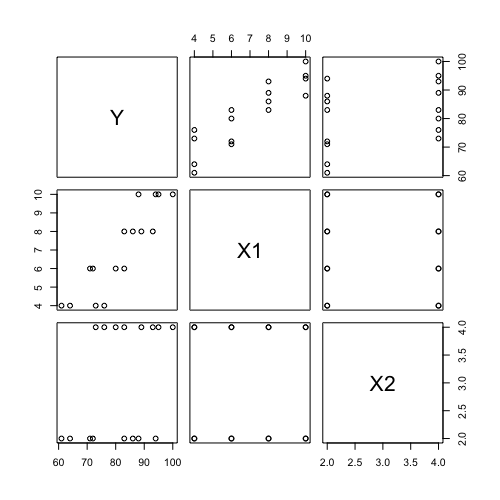
\includegraphics[width=.5\linewidth]{p1/5a.png}
		\vspace{-5ex}
	\end{figure}
	Correlation matrix:
	\lstinputlisting{p1/5a.txt}
	From the scatter plot matrix, we can see there is a strong correlation between $Y$ and $X_1$. From the correlation matrix, we can see that the correlation between $Y$ and $X_1$ are stronger than that between $Y$ and $X_2$ ($0.89>0.39$). Also, there is no linear correlation between $X_1$ and $X_2$ since the correlation is 0.
	
	\item [b.]
	Fit regression model (6.1) to the data. State the estimated regression function. How is $b_1$ interpreted here?
	
	After fitting regression model to the data, we obtain the following coefficients:
	\lstinputlisting{p1/5b.txt}
	So, the estimated regression function is $\hat{Y} = 37.65 + 4.425 x_1 + 4.375 x_2$. The interpretation is that when sweetness ($X_2$) is fixed, the brand liking ($Y$) will increase by $b_1 = 4.425$ units if mosture content ($X_1$) increases by 1 unit.
	
	\item [c.]
	Obtain the residuals and prepare a box plot of the residuals. What information does this plot provide?
	
	The residuals are
	\lstinputlisting{p1/5c.txt}
	Box plot of the residuals:
	\begin{figure}[H]
		\centering
		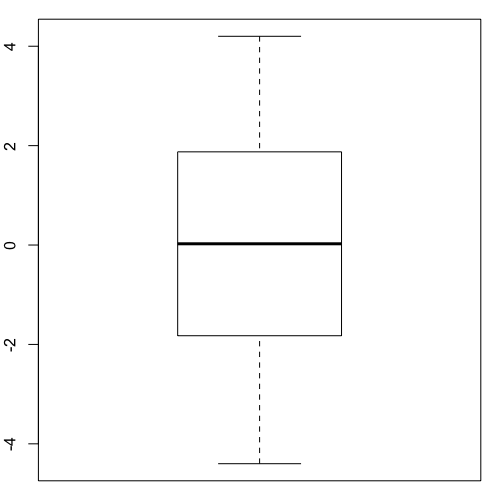
\includegraphics[width=.35\linewidth]{p1/5c.png}
	\end{figure}
	The plot shows that the residuals are symmetrically centered around 0.
	
	\item [d.]
	Plot the residuals against $\hat{Y}, X_1, X_2$ and $X_1 X_2$ on separate graphs. Also prepare a normal probability plot. Interpret the plots and summerize your findings.
	\begin{figure}[H]
		\centering
		\begin{subfigure}[b]{.4\linewidth}
			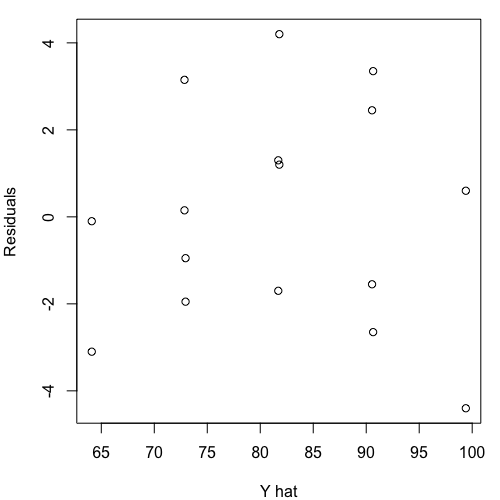
\includegraphics[width=\linewidth]{p1/5d1.png}
		\end{subfigure}
		\begin{subfigure}[b]{.4\linewidth}
			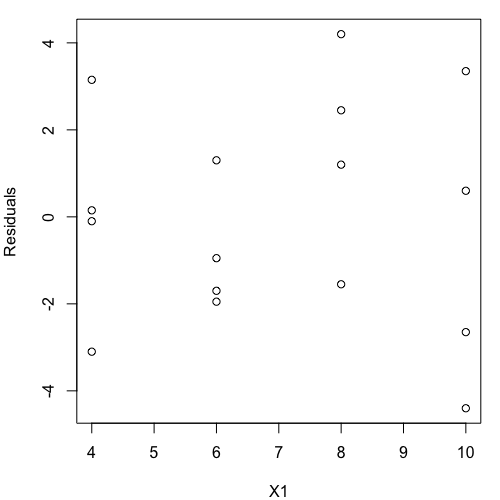
\includegraphics[width=\linewidth]{p1/5d2.png} 
		\end{subfigure}\\
		\begin{subfigure}[b]{.4\linewidth}
			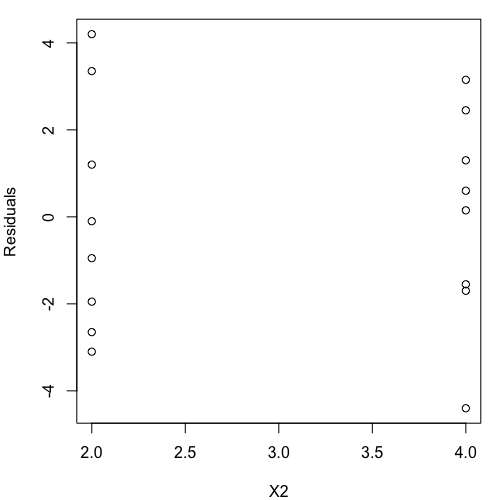
\includegraphics[width=\linewidth]{p1/5d3.png} 
		\end{subfigure}
		\begin{subfigure}[b]{.4\linewidth}
			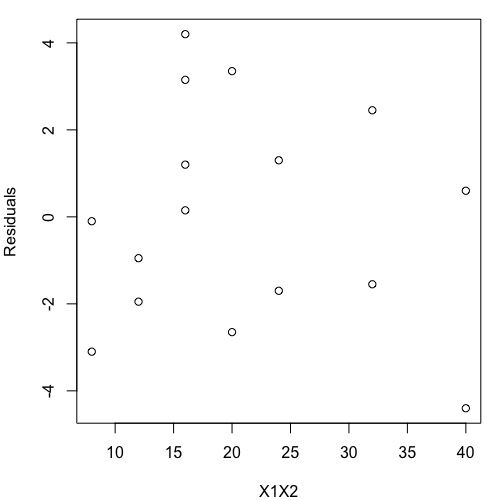
\includegraphics[width=\linewidth]{p1/5d4.png} 
		\end{subfigure} 
	\end{figure}
	There are no linear relationships shown in the plots above, indicating constancy of error variance and that the model fits the data well. The plot of residuals against $X_1 X_2$ indicates there is no interaction effect present. 
	\begin{figure}[H]
		\centering
		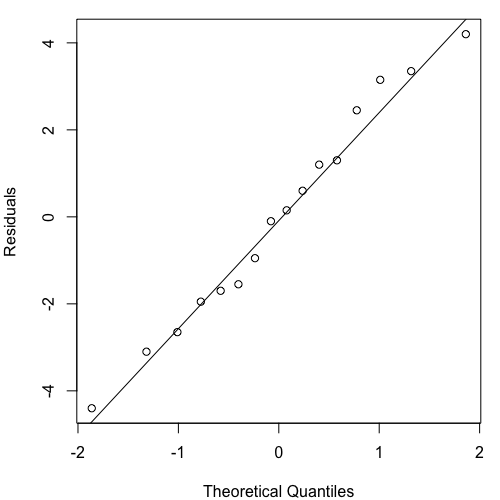
\includegraphics[width=.5\linewidth]{p1/5dqq.png}
	\end{figure}
	The normal QQ-plot above shows a strong linear correlation, confirming that the error terms are fairly normally distributed.
	
	\item [e.]
	Conduct the Breusch-Pagan test for constancy of the error variance, assuming $\log \sigma_i^2 = \gamma_0 + \gamma_1 X_{i1} + \gamma_2 X_{i2}$; use $\alpha = .01$. State the alternatives, decision rule, and conclusion.
	
	The alternatives are
	\begin{align*}
		H_0 &: \gamma_1 = \gamma_2 = 0\\
		H_a &: \gamma_1 \ne 0 \text{ or } \gamma_2 \ne 0
	\end{align*}
	The BP-statistic is
	\[
	\chi^2_{BP} = \frac{SSR^*}{p} \div \pa{\frac{SSE}{n}}^2
	\]
	where $SSR^*$ is the regression sum of squares when regressing $e^2$ on $X$.
	The decision rule is
	\begin{align*}
	\text{If } \chi^2_{BP} \le \chi^2(0.99; 2) = 9.21034, \text{ conclude } H_0\\
	\text{If } \chi^2_{BP} > \chi^2(0.99; 2) = 9.21034, \text{ conclude } H_a
	\end{align*}
	According to the ANOVA tables of two models, we have
	\[
	\chi^2_{BP} = \frac{67.34+5.06}{2} \div \pa{\frac{94.30}{16}}^2 = 1.042138 < 9.21034
	\]
	Therefore, we conclude $H_0$, that the error variance is constant.
	
	\item [f.]
	Conduct a formal test for lack of fit of the first-order regression function; use $\alpha = .01$. State the alternatives, decision rule, and conclusion.
	
	The alternatives are
	\begin{align*}
		H_0 &: E(Y) = \beta_0 + \beta_1 X_1 + \beta_2 X_2 \\
		H_a &: E(Y) \ne \beta_0 + \beta_1 X_1 + \beta_2 X_2
	\end{align*}
	The test statistic is
	\[
	F^* = \frac{SSLF}{c-2} \div \frac{SSPE}{n-c}
	\]
	The decision rule is
	\begin{align*}
		\text{If } F^* \le F(1-\alpha; c-2, n-c) = 6.370681, \text{ conclude } H_0\\
		\text{If } F^* > F(1-\alpha; c-2, n-c) = 6.370681, \text{ conclude } H_a
	\end{align*}
	The ANOVA table is shown below:
	\lstinputlisting{p1/5f.txt}
	From the table, we have $F^* = (37.30/5)/(57.00/8) = 1.047018 < 6.370681$. So, we conclude $H_0$, that $E(Y) = \beta_0 + \beta_1 X_1 + \beta_2 X_2$.
	
\end{enumerate}

\section*{Problem 2}
(Ex. 6.18) \textbf{Commercial properties}
\begin{enumerate}
	\item [a.]
	Prepare a stem-and-leaf plot for each predictor variable. What information do these plots provide?
	
	Stem-and-leaf plot for $X_1$:
	\lstinputlisting{p2/18a1.txt}
	Stem-and-leaf plot for $X_2$:
	\lstinputlisting{p2/18a2.txt}
	Stem-and-leaf plot for $X_3$:
	\lstinputlisting{p2/18a3.txt}
	Stem-and-leaf plot for $X_4$:
	\lstinputlisting{p2/18a4.txt}
	From the plots, we can see that $X_1$ ranges from 0 to 20, $X_2$ ranges from 2 to 14.6, $X_3$ ranges from 0 to 0.73 and mostly takes value less than 0.1, $X_4$ ranges from 30000 to 480000.
	
	\item [b.]
	Obtain the scatter plot matrix and the correlation matrix. Interpret these and state your principal findings.
	
	Scatter plot matrix:
	\begin{figure}[H]
		\centering
		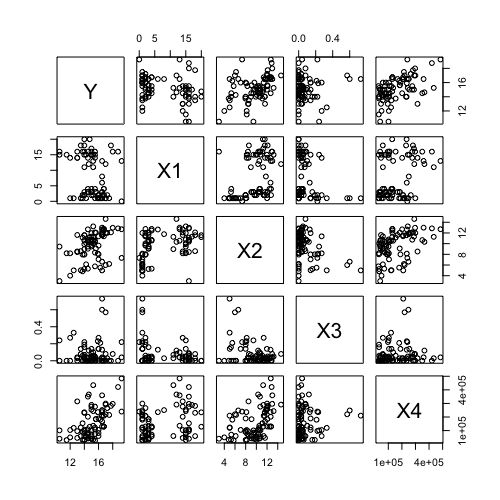
\includegraphics[width=.65\linewidth]{p2/18b.png}
	\end{figure}
	Correlation matrix:
	\lstinputlisting{p2/18b.txt}
	The scatter plot matrix shows the relationships among the variables and the correlation matrix provides the corelation coefficients. We can see that there is no strong linear correlation among the variables, but the correlation between $Y$ and $X_2$, and also the correlation between $Y$ and $X_4$, are relatively high.
	
	\item [c.]
	Fit regression model (6.5) for four predictor variables to the data. State the estimated regression function. 
	
	After fitting regression model to the data, we obtain the following coefficients:
	\lstinputlisting{p2/18c.txt}
	So, the estimated regression function is $\hat{Y} = 12.2 - 0.142 x_1 + 0.282 x_2 + 0.619 x_3 + 0.00000792 x_4$.
	
	\item [d.]
	Obtain the residuals and prepare a box plot of the residuals. Does the distribution appear to be fairly symmetrical?
	
	The residuals are in the residuals list of the model. Below is the box plot of the residuals:
	\begin{figure}[H]
		\centering
		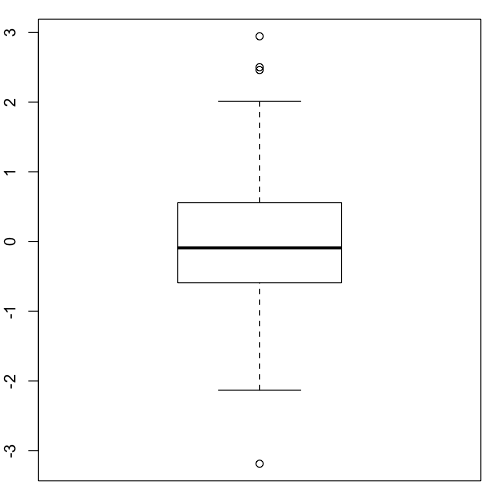
\includegraphics[width=.4\linewidth]{p2/18d.png}
	\end{figure}
	The distribution appears to be fairly symmetrical. Just a few outliners.
	
	\item [e.]
	Plot the residuals against $\hat{Y}$, each predictor variable, and each two-factor interaction term on separate graphs. Also prepare a normal probability plot. Analyze your plots and summerize your findings.
	
	\begin{figure}[H]
		\centering
		\begin{subfigure}[b]{.25\linewidth}
			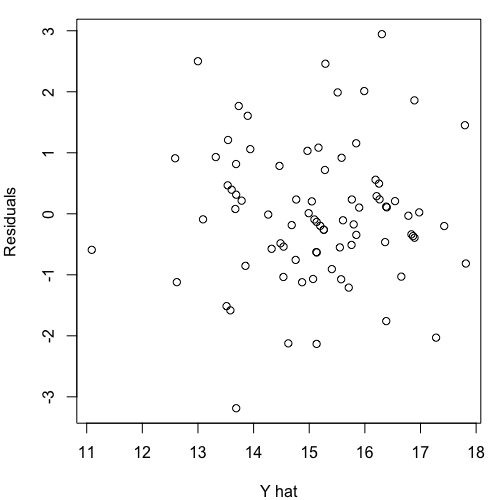
\includegraphics[width=\linewidth]{p2/18e_yhat.png}
		\end{subfigure}%%
		\begin{subfigure}[b]{.25\linewidth}
			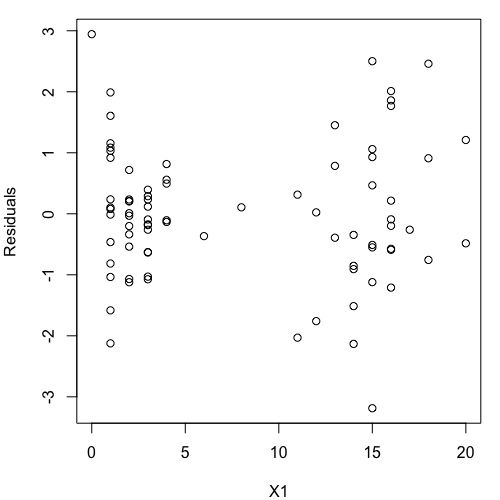
\includegraphics[width=\linewidth]{p2/18e_x1.png} 
		\end{subfigure}%%
		\begin{subfigure}[b]{.25\linewidth}
			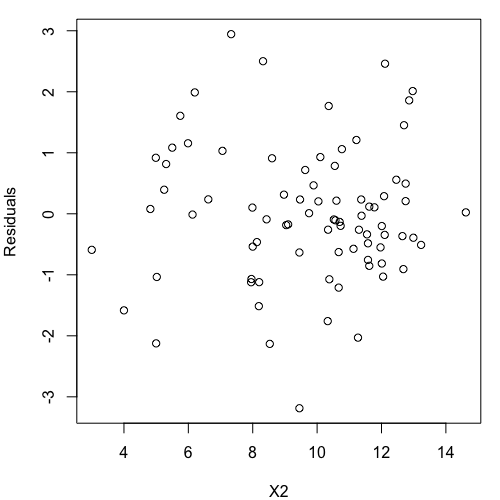
\includegraphics[width=\linewidth]{p2/18e_x2.png} 
		\end{subfigure}%%
		\begin{subfigure}[b]{.25\linewidth}
			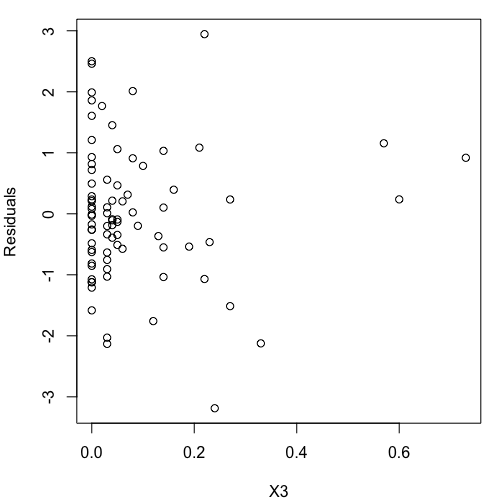
\includegraphics[width=\linewidth]{p2/18e_x3.png} 
		\end{subfigure}\\
		\begin{subfigure}[b]{.25\linewidth}
			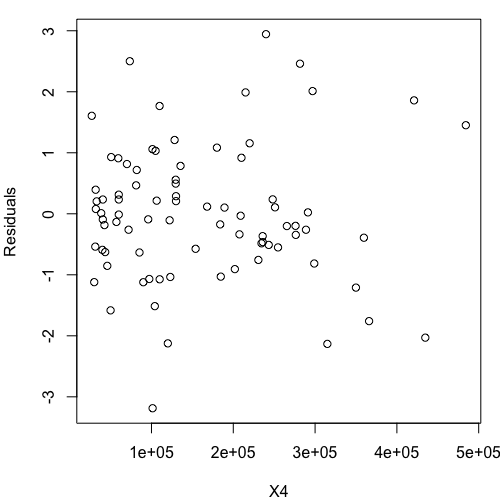
\includegraphics[width=\linewidth]{p2/18e_x4.png}
		\end{subfigure}%%
		\begin{subfigure}[b]{.25\linewidth}
			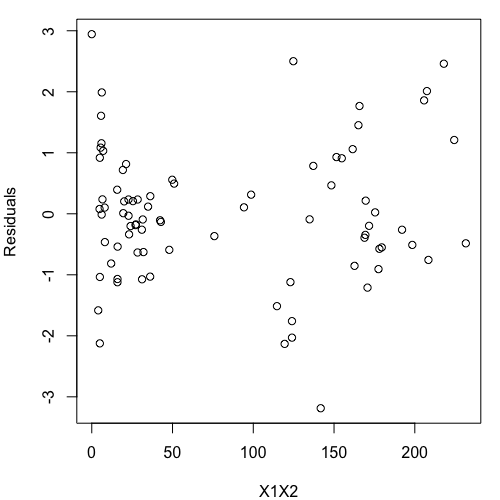
\includegraphics[width=\linewidth]{p2/18e_x1x2.png} 
		\end{subfigure}%%
		\begin{subfigure}[b]{.25\linewidth}
			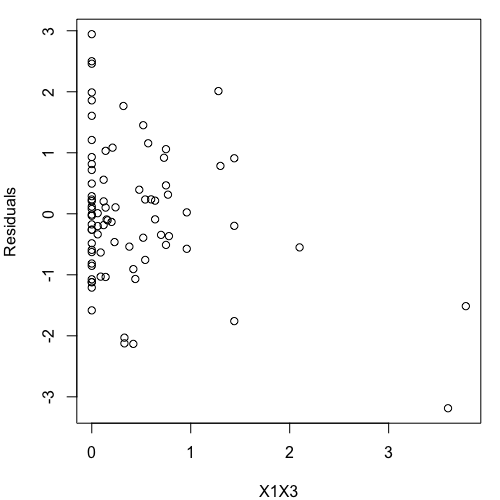
\includegraphics[width=\linewidth]{p2/18e_x1x3.png} 
		\end{subfigure}%%
		\begin{subfigure}[b]{.25\linewidth}
			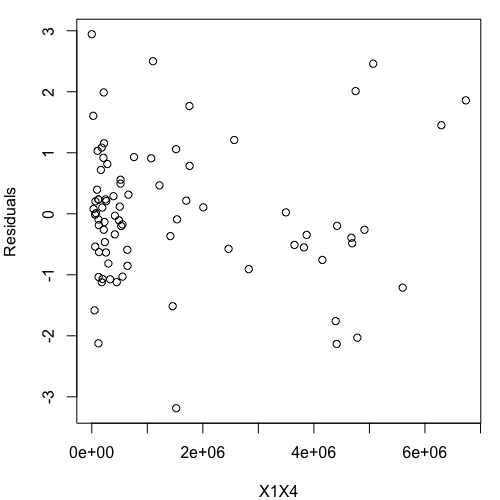
\includegraphics[width=\linewidth]{p2/18e_x1x4.png} 
		\end{subfigure}\\
		\begin{subfigure}[b]{.25\linewidth}
			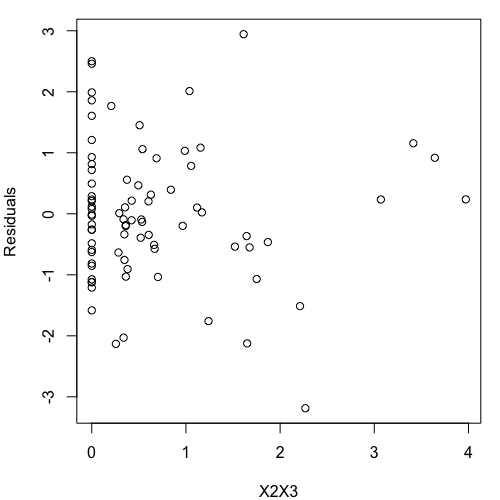
\includegraphics[width=\linewidth]{p2/18e_x2x3.png}
		\end{subfigure}%%
		\begin{subfigure}[b]{.25\linewidth}
			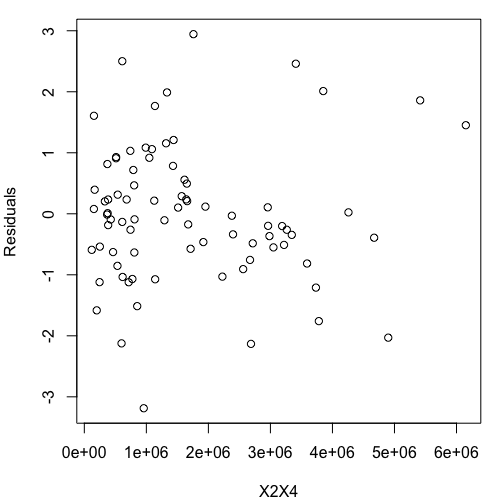
\includegraphics[width=\linewidth]{p2/18e_x2x4.png} 
		\end{subfigure}%%
		\begin{subfigure}[b]{.25\linewidth}
			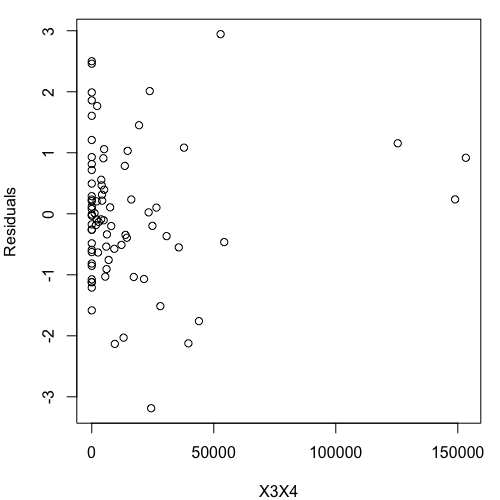
\includegraphics[width=\linewidth]{p2/18e_x3x4.png} 
		\end{subfigure}%%
		\begin{subfigure}[b]{.25\linewidth}
			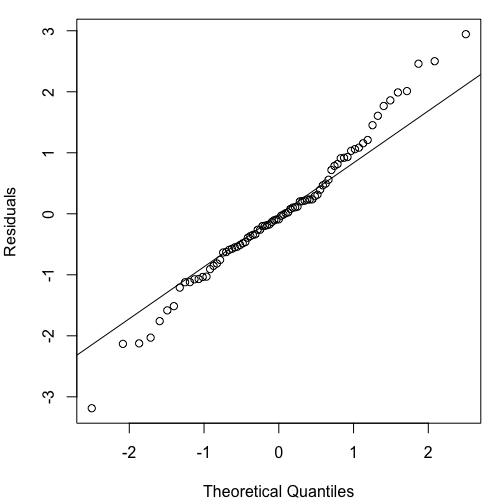
\includegraphics[width=\linewidth]{p2/18eqq.png} 
		\end{subfigure}
	\end{figure}
	In the plots with $x$-axis representing $X_3, X_1 X_3, X_2 X_3$ and $X_3 X_4$, the residuals are getting more concentrated around 0 as the predictors increase. The S shape in the QQ-plot indicates the error is not normally distributed.
	
	\item [f.]
	Can you conduct a formal test for lack of fit here?
	
	No, because there are no observations with the same values of predictor variables.
	
	\item [g.]
	Divide the 81 cases into two groups, placing the 40 cases with the smallest fitted values $\hat{Y}_i$ into group 1 and the remaining cases into group 2. Conduct the Brown-Forsythe test for constancy of the error variance, using $\alpha = .05$. State the decision rule and conclusion.
	
	The alternatives are
	\begin{align*}
		H_0 &: \text{error variance is constant}\\
		H_a &: \text{error variance is not constant}
	\end{align*}
	The test statistic is
	\[
	t_{BF}^* = \frac{\bar{d}_1 - \bar{d}_2}{s\sqrt{\frac{1}{n_1} + \frac{1}{n_2}}}
	\]
	The decision rule is
	\begin{align*}
		\text{If } t_{BF}^* \le t(1-\alpha/2; n-2) = 1.99045, \text{ conclude } H_0\\
		\text{If } t_{BF}^* > t(1-\alpha/2; n-2) = 1.99045, \text{ conclude } H_a
	\end{align*}
	We can obtain $s$ from the pooled variance,
	\[
	s = \sqrt{\frac{\sum (d_{i1} - \bar{d}_1) + \sum (d_{i2} - \bar{d}_2)}{n-2}} = \sqrt{\frac{20.3091 + 22.4447}{81-2}} = 0.7357
	\]
	Then the test statistic is given by
	\[
	t_{BF}^* = \frac{0.8696 - 0.7793}{0.7357\sqrt{\frac{1}{40} + \frac{1}{41}}} = 0.5521
	\]
	Since $t_{BF}^* = 0.5521 < 1.99045$, we conclude $H_0$, that the error variance is constant.
	
\end{enumerate}

\section*{Problem 3}
(Ex. 6.19) Refer to \textbf{Commercial properties} Problem 6.18. Assume that regression model (6.5) for four predictor variables with independent normal error terms is appropriate.
\begin{enumerate}
	\item [a.]
	Test whether there is a regression relation; use $\alpha = .05$. State the alternatives, decision rule, and conclusion. What does your test imply about $\beta_1, \beta_2, \beta_3,$ and $\beta_4$? What is the $P$-value of the test?
	
	The alternatives are
	\begin{align*}
		H_0 &: \beta_1 = \beta_2 = \dots = \beta_{p-1} = 0\\
		H_a &: \text{not all } \beta_i=0, i=1,\dots,p-1
	\end{align*}
	The test statistic is
	\[
	F^* = \frac{MSR}{MSE}
	\]
	The decision rule is
	\begin{align*}
	\text{If } F^* \le F(1-\alpha; p-1, n-p) = 2.492049, \text{ conclude } H_0\\
	\text{If } F^* > F(1-\alpha; p-1, n-p) = 2.492049, \text{ conclude } H_a
	\end{align*}
	The ANOVA table is shown below:
	\lstinputlisting{p3/19a.txt}
	So, the test statistic $F^* = \frac{(14.819+72.802+8.381+42.325)/4}{98.231/76} = 26.75543 > 2.492049$, we conclude $H_a$, that not all $\beta_i$ is zero. The $P$-value is $7.272e-14$.
	
	\item [b.]
	Estimate $\beta_1, \beta_2, \beta_3,$ and $\beta_4$ jointly by the Bonferroni procedure, using a 95 percent family confidence coefficient. Interpret your results.
	
	We can obtain the standard errors of $\hat{\beta}_i$ from the summary table below:
	\lstinputlisting{p3/19b.txt}
	The confidence limits with family confidence coefficient 0.95 are
	\[
	\hat{\beta}_i \pm B\cdot s\{\hat{\beta}_i\}
	\]
	where $B = t(1-\alpha/2g; n-p) = t(0.99375; 76) = 2.558541$. So, the Bonferroni 95\% joint CIs for $\beta_1, \beta_2, \beta_3,$ and $\beta_4$ are
	\begin{align*}
		\beta_1 &: -0.142034 \pm 2.558541 \cdot 0.021343 = (-0.196641, -0.087427)\\
		\beta_2 &: 0.282017 \pm 2.558541 \cdot 0.063172 = (0.1203888, 0.443645)\\
		\beta_3 &: 0.619344 \pm 2.558541 \cdot 1.086813 = (-2.161312, 3.4)\\
		\beta_4 &: 0.000008 \pm 2.558541 \cdot 0.000001 = (0.000004, 0.000011)
	\end{align*}
	meaning that we are 95\% confident the $\beta_i$'s will fall in the intervals simultaneously.
	
	\item [c.]
	Calculate $R^2$ and interpret this measure.
	
	From the ANOVA table, we have
	\[
	R^2 = \frac{SSR}{SSTO} = \frac{14.819+72.802+8.381+42.325}{14.819+72.802+8.381+42.325+98.231} = \frac{138.327}{236.558} = 0.584749
	\]
	It measures the proportionate reduction of total variation in $Y$ associated with the use the set of $X$ variables.
\end{enumerate}

\section*{Problem 4}
(Ex. 6.20) Refer to \textbf{Commercial properties} Problem 6.18. Assume that regression model (6.5) for four predictor variables with independent normal error terms is appropriate. The researcher wishes to obtain simultaneous interval estimates of the mean rental rates for four typical properties specified as follows:
\begin{table}[H]
	\centering
	\begin{tabular}{*{5}{N}}
		& 1 & 2 & 3 & 4 \\ \midrule
		X_1: & 5.0 & 6.0 & 14.0 & 12.0 \\
		X_2: & 8.25 & 8.50 & 11.50 & 10.25 \\
		X_3: & 0 & 0.23 & 0.11 & 0 \\
		X_4: & 250000 & 270000 & 300000 & 310000 \\
	\end{tabular}
\end{table}
Obtain the family of estimates using a 95 percent family confidence coefficient. Employ the most efficient procedure.

Applying Bonferroni procedure, we have 
\[
B = t(1-\alpha/2g; n-p) = t(0.99375; 76) = 2.558541
\]
So the CIs are
\begin{align*}
	Y_{h1} &: \hat{Y}_{h1} \pm B\hat{\sigma} \sqrt{x_{h1}' (X'X)^{-1} x_{h1}^{}} = 15.79813 \pm 2.558541 \cdot 1.137102 \cdot 0.244601 = (15.08651, 16.50975)\\
	Y_{h2} &: \hat{Y}_{h2} \pm B\hat{\sigma} \sqrt{x_{h2}' (X'X)^{-1} x_{h2}^{}} = 16.02754 \pm 2.558541 \cdot 1.137102 \cdot 0.207519 = (15.4238, 16.63128)\\
	Y_{h3} &: \hat{Y}_{h3} \pm B\hat{\sigma} \sqrt{x_{h3}' (X'X)^{-1} x_{h3}^{}} = 15.90072 \pm 2.558541 \cdot 1.137102 \cdot 0.195411 = (15.33221, 16.46923)\\
	Y_{h4} &: \hat{Y}_{h4} \pm B\hat{\sigma} \sqrt{x_{h4}' (X'X)^{-1} x_{h4}^{}} = 15.84339 \pm 2.558541 \cdot 1.137102 \cdot 0.227928 = (15.18027, 16.50651)
\end{align*}

\section*{Problem 5}
Suppose that $\m{X}= [\m{x}_1, \dots, \m{x}_k]$, where $\m{x}_i$, $i=1, \dots k$ are linearly independent columns of $\m{X}$ (one of $\m{x}_i$ can be a column of $\m{1}$ if intercept is included in the model). Show that $\var(\hat{\beta}_k) \ge \sigma^2(\m{x}_k' \m{x}_k)^{-1}$ with equality if and only if $\m{x}_k' \m{x}_j = 0, j=0,1,\dots,k-1$.

Since $\var(\hat{\beta}_k) = \sigma^2 \pa{\m{X}' \m{X}}^{-1}_{k,k}$, 
\begin{align*}
\var(\hat{\beta}_k) \ge \sigma^2(\m{x}_k' \m{x}_k)^{-1} 
&\Leftrightarrow 
\sigma^2 \pa{\m{X}' \m{X}}^{-1}_{k,k} \ge \sigma^2(\m{x}_k' \m{x}_k)^{-1}\\
&\Leftrightarrow 
\pa{\m{X}' \m{X}}^{-1}_{k,k} \ge (\m{x}_k' \m{x}_k)^{-1}
\end{align*}
\iffalse
Partition $\m{X}$ into two blocks then we have
\[
\m{X} = 
	\left[
	\begin{array}{c}
	\m{X}_{-k}\\ \hline
	\m{x}'_k
	\end{array}
	\right]
,
\m{X}' =
	\left[
	\begin{array}{c|c}
	\m{X}'_{-k} & \m{x}_k
	\end{array}
	\right]
\]
where $\m{x}_k$ is the $k$-th row of $\m{X}$, and $\m{X}_{-k}$ is the matrix with $\m{x}_k$ removed. By block matrix multiplication, we obtain
\[
\m{X}' \m{X}= \m{X}'_{-k} \m{X}_{-k} + \m{x}_k \m{x}'_k
\]
\fi
Dividing $\m{X}' \m{X}$ into four blocks, we have
\[
\m{X}' \m{X} =
	\left[
	\begin{array}{c|c}
	A & B \\ \hline
	B' & C
	\end{array}
	\right]
\]
where $C_{1\times1} = \m{x}_k' \m{x}_k$. Taking the inverse of $\m{X}' \m{X}$,
\[
(\m{X}' \m{X})^{-1} = 
	\left[
	\begin{array}{c|c}
	D & E \\ \hline
	E' & F
	\end{array}
	\right]
\]
According to a theorem of inverse of a partitioned symmetric matrix, 
\[
F = (C - B'A^{-1}B)^{-1} = C^{-1} + C^{-1}B'(A-BC^{-1}B')^{-1} BC^{-1}
\]
Substitute $C= \m{x}_k' \m{x}_k$ into the equation above
\begin{align*}
	\pa{\m{X}' \m{X}}^{-1}_{k,k} 
	&= F\\
	&= C^{-1} + C^{-1}B'(A-BC^{-1}B')^{-1} BC^{-1}\\
	&= (\m{x}_k' \m{x}_k)^{-1} + (\m{x}_k' \m{x}_k)^{-1} B'(A-B(\m{x}_k' \m{x}_k)^{-1}B')^{-1} B(\m{x}_k' \m{x}_k)^{-1}
\end{align*}
Because $\m{x}_k' \m{x}_k$ represents the sum of square of the $k$-th column, $\m{x}_k' \m{x}_k\ge 0$, and $(\m{x}_k' \m{x}_k)^{-1}\ge 0$. 
Since $\m{x}_i$ are linearly independent columns, and $(\m{x}_k' \m{x}_k)^{-1}\ge 0$, $(\m{x}_k' \m{x}_k)^{-1} B'(A-B(\m{x}_k' \m{x}_k)^{-1}B')^{-1} B(\m{x}_k' \m{x}_k)^{-1}\ge 0$; so $\pa{\m{X}' \m{X}}^{-1}_{k,k} \ge (\m{x}_k' \m{x}_k)^{-1}$. 
Because $B = [\m{x}_1, \m{x}_2, \dots ,\m{x}_{k-1}]'\m{x}_k$ and $B' = \m{x}'_k [\m{x}_1, \m{x}_2, \dots ,\m{x}_{k-1}]$, $B=B'=\m{0}$ if and only $\m{x}_k' \m{x}_j = 0$ for $j=0,1,\dots,k-1$; with $B=B'=\m{0}$, $\pa{\m{X}' \m{X}}^{-1}_{k,k} = (\m{x}_k' \m{x}_k)^{-1}$. 
Therefore, by proving $\pa{\m{X}' \m{X}}^{-1}_{k,k} \ge (\m{x}_k' \m{x}_k)^{-1}$ with equality if and only if $\m{x}_k' \m{x}_j = 0, j=0,1,\dots,k-1$, we show that $\var(\hat{\beta}_k) \ge \sigma^2(\m{x}_k' \m{x}_k)^{-1}$ with equality if and only if $\m{x}_k' \m{x}_j = 0, j=0,1,\dots,k-1$.
\end{document}

